\documentclass{article}
\usepackage[preprint]{caisc_2026}
\usepackage[utf8]{inputenc}
\usepackage[T1]{fontenc}
\usepackage{hyperref}
\usepackage{url}
\usepackage{booktabs}
\usepackage{amsfonts}
\usepackage{amsmath}
\usepackage{microtype}
\usepackage{xcolor}
\usepackage{graphicx}

% --- numbers filled from the calibrated runs (src/pmut_echo_sim.py) ---
\newcommand{\snrA}{+33}     % 100 kHz
\newcommand{\snrB}{+14}     % 135 kHz
\newcommand{\snrC}{-33}     % 200 kHz
\newcommand{\echoA}{479\,mV}
\newcommand{\echoB}{57.6\,mV}
\newcommand{\echoC}{0.316\,mV}
\newcommand{\oilA}{11}      % dB round trip 75 kHz (approx)
\newcommand{\oilB}{120}     % dB round trip 250 kHz
\newcommand{\oilC}{1920}    % dB round trip 1 MHz
\newcommand{\Cs}{479\,nF}
\newcommand{\en}{4\,nV/\!\sqrt{\text{Hz}}}
\newcommand{\sqRecip}{27}   % fC/Pa
\newcommand{\sqEq}{1130}    % fC/Pa
\newcommand{\fbound}{135}   % kHz detection boundary
\newcommand{\Wtx}{55\,mW}
\newcommand{\Pface}{254\,kPa}
\newcommand{\faceVel}{5.5\,mm/s}
\newcommand{\fillDB}{-28.9}
\newcommand{\gainMax}{0.77}

\title{Modelling of a PMUT Pulse-Echo Through an Oil-Filled Steel Tube}

\author{%
  Jyotirmoy Ray \\
  Wipro Research \\
  \texttt{jyotirmoy.ray@wiproresearch.in}
}

\begin{document}
\maketitle

\begin{abstract}
Piezoelectric micromachined ultrasonic transducers (PMUTs) are usually designed for
short-range imaging in soft tissue near 1\,MHz. I ask a different question: can a PMUT
range a target by pulse-echo down a 3\,m oil-filled steel tube, and what actually limits
it? Starting from the published system-level transducer model of Dangi and Pratap (2017),
which radiates into air over sub-half-metre distances and carries no noise model, I add
the missing pieces: an acoustic-channel model for the tube treated as a waveguide
(transfer-matrix wall coupling, confinement instead of spherical spreading, frequency
dependent oil absorption, and a near-total far-end reflector), a first-principles
charge-amplifier receiver-noise model, and a two-dimensional finite-difference wave
simulation for visualization. Three results emerge that overturn the default intuition.
First, the conventional choice of frequency is backwards: oil absorption scales as
$f^2$ over the fixed round trip, so the echo amplitude collapses as $\exp(-k f^2)$, giving
\oilC\,dB of round-trip loss at 1\,MHz versus \oilB\,dB at 250\,kHz; the usable band lies
near and below \fbound\,kHz, not at 1\,MHz. Second, when transmit and receive are forced to
derive from one electromechanical coupling (so the two-way link is passive, which the
published sensitivities are not: they imply voltage gain above unity), the detection
boundary sits at roughly \fbound\,kHz for a representative 20\,dB/m oil. Third, the binding
constraint is the receiver, not the channel: a thin-film-PZT clamped capacitance of order
\Cs{} feeding a low-noise charge amplifier sets a noise floor tens of dB above the
convenient ``$10\,\mu$V'' placeholder. I give the link budget, the reciprocity relation, the
noise model, a 100/\fbound/200\,kHz comparison spanning detectable to buried, and matching
wave-propagation movies. Absolute signal-to-noise carries order-of-magnitude uncertainty
because the source paper's own transmit and receive sensitivities disagree by more than
$100\times$; the relative structure, the cliff, and the receiver-limited regime are robust.
\end{abstract}

\section{Introduction}
Ultrasonic ranging through metal walls and along fluid-filled tubes is attractive for
level sensing, leak and blockage detection, and through-wall telemetry in sealed vessels.
Piezoelectric micromachined ultrasonic transducers (PMUTs) are small, low-power, and
CMOS-compatible, which makes them appealing for such embedded sensing~\citep{jung2017,przybyla2011}. Almost all PMUT
design practice, however, targets short-range medical and fingerprint imaging, where the
operating frequency is pushed toward 1\,MHz and above to improve axial resolution, and
where the propagation medium is soft tissue or water over millimetres to a few centimetres.

The question that motivates this work is whether that design point transfers to a very
different regime: a transducer at one end of a 3\,m oil-filled steel tube, attempting to
detect the echo from the far end. The starting point is the system-level analytical model
of \citet{dangi2017}, which compactly relates a multilayer PMUT's transmit
pressure, receive charge, and quality factor to its geometry through three nearly invariant
mode-shape factors. That model is validated for radiation into air over distances below
0.5\,m and contains no treatment of layered solid/liquid channels, of propagation to metres,
of pulse-echo, or of noise. It therefore cannot, by itself, answer the ranging question.

I extend it into an end-to-end link model and report three findings. (1) The operating
frequency is set by a steep absorption cliff: because the oil attenuation coefficient grows
as $f^2$, the round-trip loss over 6\,m is \oilA\,dB at 75\,kHz, \oilB\,dB at 250\,kHz, and
\oilC\,dB at 1\,MHz; the intuitive high-frequency choice is not merely suboptimal but
fatal, and the usable band is far lower. (2) Confinement, not radiation, governs feasibility:
the tube is a waveguide, so the spherical spreading that dominates a free-field budget is
replaced by a bounded cross-section fill loss. (3) When the transmit and receive paths are
required to come from a single coupling so the link is passive, and noise is modeled from the
transducer capacitance and amplifier rather than assumed, the detection boundary lands near
\fbound\,kHz and is set by the receiver electronics rather than by the acoustic channel.

My contribution is a careful, reciprocity-consistent system model and the resulting design
inferences, not a new transducer or a new experiment. I am explicit about a calibration
caveat: the source paper's published transmit and receive sensitivities are mutually
inconsistent by more than two orders of magnitude, so absolute signal-to-noise ratios (SNRs)
are uncertain to within roughly that factor. The robust outputs are the relative trends,
the $f^2$ cliff, the passivity constraint, and the receiver-limited regime, all of which are
independent of the absolute calibration.

\section{Background: the starting transducer model}
A PMUT is a clamped circular multilayer plate with a piezoelectric layer (here lead
zirconate titanate, PZT) between electrodes on a passive structural layer. Applying a
voltage produces an unbalanced in-plane stress and hence a bending moment, so the plate
vibrates flexurally and pumps the adjacent fluid; conversely an incident pressure flexes the
plate and generates charge. \citet{dangi2017}, building on the natural-frequency derivation of \citet{sammaoura2012}, reduce this to a lumped
electro-mechano-acoustic circuit and obtain closed forms for the first-mode natural
frequency, the receive charge sensitivity (their Eq.~17), the transmit response, and the
quality factor, all written through three mode-shape participation factors
$\Lambda', \Lambda_1, \Lambda_2$ that vary little across designs. I reuse those relations
for the transducer and treat everything outside the device, the channel and the receiver
electronics, as the part to be built. Section~\ref{sec:transducer} returns to a subtlety in
how the transmit and receive sides of that model must be coupled.

\section{System model}\label{sec:model}
Figure~\ref{fig:schematic} shows the geometry. A PMUT (or, more realistically, a small
PMUT array forming an effective aperture of radius $a_{\mathrm{ap}}$) sits at the near end of
a steel tube of outer diameter 300\,mm and wall thickness 10\,mm, so the inner oil radius is
$R_{\mathrm{in}}=140$\,mm. The tube is filled with a synthetic mineral oil and is
$L=3$\,m long. The far end is a thick steel block, thick enough that the steel/air interface
behind it is irrelevant, so it acts as a near-total acoustic reflector. The transducer both
transmits and, after the round trip, receives.

\begin{figure}[t]
\centering
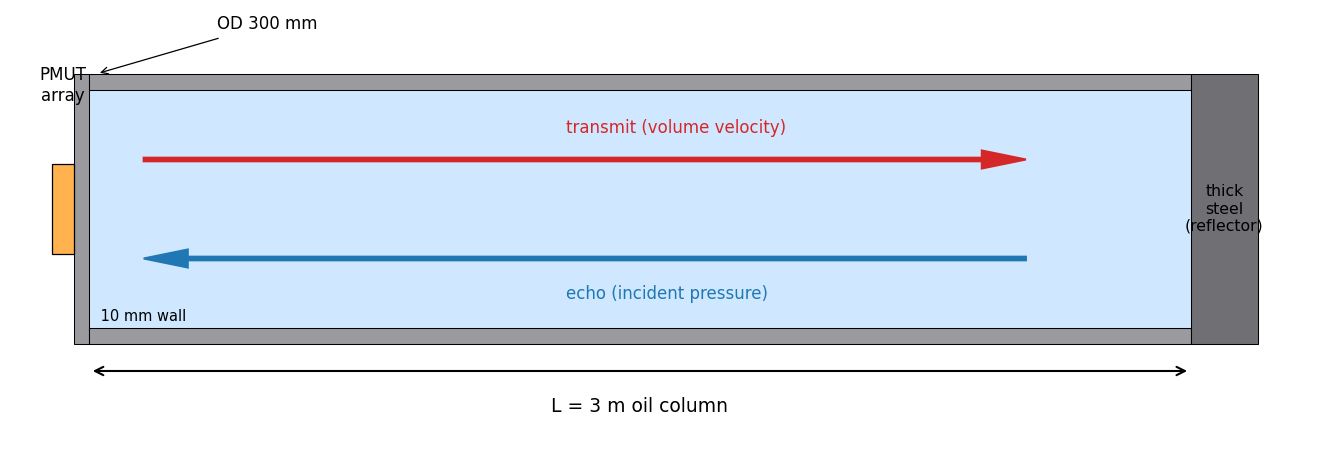
\includegraphics[width=0.92\linewidth]{../figures/fig_schematic.png}
\caption{Pulse-echo geometry. A PMUT array at the near end launches into the oil column
through the 10\,mm steel end-cap; the wave travels 3\,m, reflects off the thick-steel far
end, and returns to the same transducer. The tube walls confine the beam, so the channel is
a waveguide rather than free space.}
\label{fig:schematic}
\end{figure}

\subsection{Acoustic channel as a link budget}
I track acoustic intensity through the round trip as a product of factors, then convert to
an incident pressure at the receiver. The transmitted power crosses the near steel cap into
the oil, propagates and attenuates to the far end, reflects, returns, and crosses the cap
again. Writing each stage as an intensity factor,
\begin{equation}
I_{\mathrm{back}} = I_{\mathrm{face}}\cdot
\underbrace{\tau_{\mathrm{wall}}}_{\text{out}}\cdot
\underbrace{\Big(\tfrac{a_{\mathrm{ap}}}{R_{\mathrm{in}}}\Big)^2}_{\text{fill}}\cdot
\underbrace{\Gamma^2}_{\text{far end}}\cdot
\underbrace{e^{-2\alpha(f)\,(2L)}}_{\text{oil absorption}}\cdot
\underbrace{\tau_{\mathrm{wall}}}_{\text{return}} .
\label{eq:linkbudget}
\end{equation}
Three of these terms carry the physics. The wall term $\tau_{\mathrm{wall}}$ is the intensity
transmission of the 10\,mm steel layer, computed from the standard single-layer acoustic
transfer matrix between the transducer-side medium and the oil; for a well-coupled (bonded)
transducer it is a flat $-10$\,dB per crossing, while for a dry, air-backed transducer it
develops deep resonance windows at multiples of $c_{\mathrm{steel}}/2d$. The confinement term
replaces free-field spherical spreading: in an unbounded fluid the round-trip on-axis pressure
falls as the square of $a^2/(\lambda z)$, costing about $-41$\,dB at 3\,m, but in the tube the
energy that fills the cross-section is conserved and the only geometric loss is the fraction
$(a_{\mathrm{ap}}/R_{\mathrm{in}})^2$ that the receive aperture re-samples, here \fillDB\,dB,
and falling to 0\,dB as the aperture fills the tube. The absorption term uses the classical
thermoviscous law~\citep{kinsler2000} in which the coefficient grows quadratically with frequency,
\begin{equation}
\alpha_{\mathrm{dB}}(f) = \alpha_0\,(f/f_{\mathrm{ref}})^2,\qquad
\alpha_0 = 20\ \text{dB/m at } f_{\mathrm{ref}}=250\,\text{kHz}.
\label{eq:absorption}
\end{equation}
This single term dominates the frequency dependence of the whole system and is the source of
the result in Section~\ref{sec:cliff}. A small additional waveguide wall-bounce loss of
0.5\,dB/m is included. The incident pressure at the receiver is
$P_{\mathrm{inc}}=\sqrt{2 Z_{\mathrm{steel}} I_{\mathrm{back}}}$.

\subsection{Reciprocity-consistent transmit and receive}\label{sec:transducer}
The error that is easy to make, and that I initially made, is to anchor the transmit and
receive paths independently: transmit from an assumed launched power, receive from the
published charge sensitivity. Doing so lets the end-to-end voltage transfer exceed unity at
low frequency (in my first runs, a 140\,V echo from a 10\,V drive), which is impossible for a
passive two-way link. The fix is to require both directions to come from one
electromechanical coupling. In the lumped model the transmit volume-velocity response and the
receive charge sensitivity share the transformer ratio $\phi$ and the mechanical impedance
$Z_m$, which forces the reciprocity relation
\begin{equation}
\left.\frac{\dot q}{V_{\mathrm{in}}}\right|_{\text{transmit}}
=\;\omega_{00}\,\left.\frac{Q}{P_{\mathrm{in}}}\right|_{\text{receive}} ,
\label{eq:reciprocity}
\end{equation}
where $\dot q$ is the volume velocity, $\omega_{00}$ the resonance, and $Q/P_{\mathrm{in}}$ the
charge per unit incident pressure. I anchor the absolute scale to the paper's \emph{measured}
transmit (a 1\,mm, 126\,kHz device deflects about 3\,nm/V at resonance, their Fig.~9) and
\emph{derive} the receive sensitivity from Eq.~\eqref{eq:reciprocity}, rather than using their
Eq.~17 in isolation. The aperture is treated as an array of elements each sized to resonate at
the operating frequency; the element count cancels in the SNR, so the result is aperture
self-consistent. With this construction the implied transmit is physically sane
(\Wtx{} launched, face velocity \faceVel, face pressure \Pface), and the two-way transfer never
exceeds $V_{\mathrm{echo}}/V_{\mathrm{in}}=\gainMax$ across the band, restoring passivity. The
reciprocity-derived receive sensitivity at 250\,kHz is \sqRecip\,fC/Pa, about $41\times$ smaller
than the paper's Eq.~17 value of \sqEq\,fC/Pa; the two published numbers are not mutually
consistent, which is the origin of the calibration caveat stated throughout.

\subsection{Receiver noise}\label{sec:noise}
The received charge is read by a charge amplifier with feedback capacitance $C_f$. The
dominant noise is the amplifier input voltage noise $e_n$ multiplied by the capacitive noise
gain $(C_{\mathrm{in}}/C_f)$, where $C_{\mathrm{in}}=C_s+C_{\mathrm{stray}}+C_f$ and $C_s$ is
the PMUT clamped capacitance. I add the amplifier current noise through the feedback
transimpedance and the PZT dielectric-loss (Johnson) noise, and integrate over the resonant
equivalent noise bandwidth $\mathrm{ENBW}=(\pi/2)(f_0/Q)$:
\begin{equation}
V_{\mathrm{noise}} = \sqrt{\,(e_n\,C_{\mathrm{in}}/C_f)^2 + (e_i\,Z_f)^2 + 4 k_B T\,G\,Z_f^2\,}\;\sqrt{\mathrm{ENBW}} .
\label{eq:noise}
\end{equation}
Thin-film PZT (650\,nm thick) over a 10\,mm aperture gives a large clamped capacitance of
order \Cs, so with a low-noise $e_n=\en$ the voltage-noise term dominates and the noise floor
is of order tens of millivolts referred to the amplifier output, far above a convenient
$10\,\mu$V placeholder. The link is therefore receiver-limited.

\section{FDTD visualization}\label{sec:fdtd}
To see the propagation I built a two-dimensional finite-difference time-domain solver on an
axial slice of the tube, following the explicit grid approach of WaveSimulator2D~\citep{wavesim2d} but using a
variable-density velocity-pressure staggered scheme~\citep{virieux1986} so that reflections follow the true
acoustic impedance $Z=\rho c$. The oil sound speed (1440\,m/s) is exact, so the round-trip
time-of-flight of about 4.17\,ms is physical. To keep the time step affordable, the steel
sound speed is reduced while its density is kept high, which preserves the impedance contrast
and hence the strong reflections; this is a visualization trade-off and the SNR numbers come
from the link budget of Section~\ref{sec:model}, not from the FDTD. Each rendered movie has
three synchronized panels: the wave field, the transmitter drive, and the received signal with
the modeled noise, plus a running readout of physical simulation time.

\section{Results}\label{sec:results}
Figure~\ref{fig:results} compares the calibrated model at 100, \fbound, and 200\,kHz, the
frequencies that bracket the detection boundary.

\begin{figure}[t]
\centering
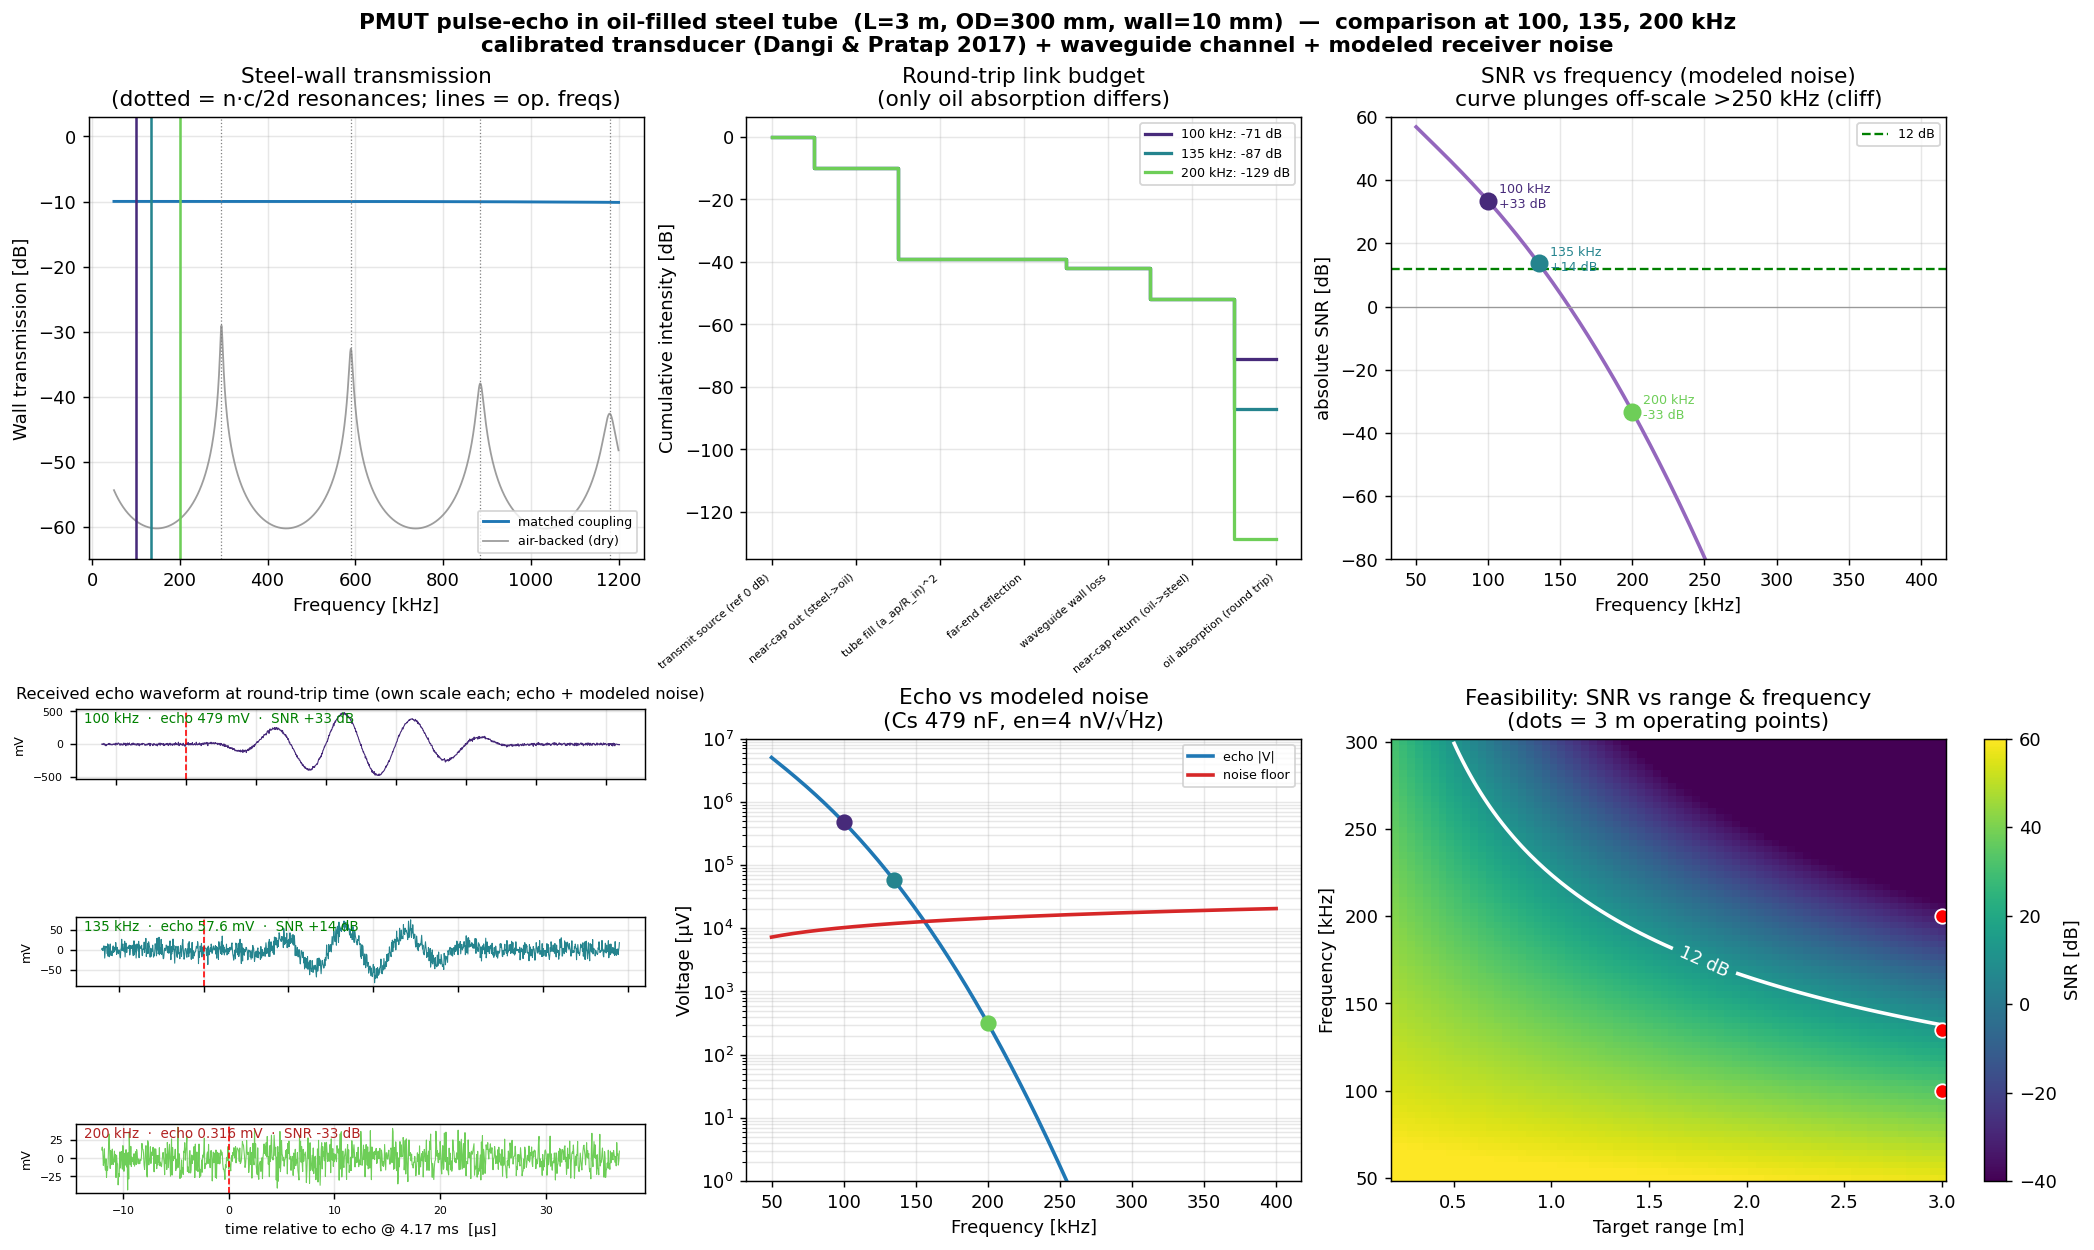
\includegraphics[width=0.99\linewidth]{../figures/pmut_tube_results.png}
\caption{Calibrated comparison at 100/\fbound/200\,kHz. (1) Steel-wall transmission: flat for
matched coupling, resonant if dry. (2) Round-trip link budget; only the oil-absorption term
differs between frequencies. (3) Absolute SNR versus frequency with the three operating points
marked; the curve plunges off-scale above 250\,kHz. (4) The actual received echo waveform plus
modeled noise at each frequency, each on its own absolute scale: a clean burst at 100\,kHz, an
echo emerging from noise at \fbound\,kHz, and pure noise at 200\,kHz. (5) Echo voltage and the
modeled noise floor versus frequency, crossing near \fbound\,kHz. (6) Feasibility map of SNR
over range and frequency, with the 12\,dB contour and the 3\,m operating points.}
\label{fig:results}
\end{figure}

\subsection{The $f^2$ absorption cliff sets the frequency}\label{sec:cliff}
Because the absorption coefficient in Eq.~\eqref{eq:absorption} grows as $f^2$, the dB loss
over the fixed 6\,m round trip also grows as $f^2$ and the echo amplitude collapses as
$\exp(-k f^2)$. The round-trip oil loss is \oilA\,dB at 75\,kHz, \oilB\,dB at 250\,kHz, and
\oilC\,dB at 1\,MHz. The receive sensitivity grows only as $1/f^2$ and the noise as
$\sqrt{f}$, so neither offsets the collapse. The practical consequence is stark and runs
against ultrasonic-imaging intuition: a frequency chosen for axial resolution is exactly the
wrong choice for long-range ranging in an absorbing liquid, and the usable band sits near and
below \fbound\,kHz. Panel~3 of Figure~\ref{fig:results} shows the cliff directly; the curve is
bounded to a readable range because past 250\,kHz it descends through hundreds of negative dB.

\subsection{A detection boundary near \fbound\,kHz}
With the reciprocity-consistent transducer and the modeled noise floor, the absolute SNRs at
the three operating points are \snrB\,dB at \fbound\,kHz, \snrA\,dB at 100\,kHz, and \snrC\,dB
at 200\,kHz, against a 12\,dB detection threshold. The received-waveform panel
(Figure~\ref{fig:results}, panel~4) tells the story in the time domain on per-frequency
absolute scales: the 100\,kHz echo is a clean \echoA{} burst well above noise, the \fbound\,kHz
echo (\echoB) just clears the noise (the knife-edge case), and the 200\,kHz echo (\echoC) is
buried. Figure~\ref{fig:montage} shows the corresponding FDTD fields: at 100\,kHz a wave packet
survives the round trip and returns to the near end, while at 200\,kHz it is absorbed in transit
and never returns. The two views, a link budget and an independent wave solve, agree on the
boundary.

\begin{figure}[t]
\centering
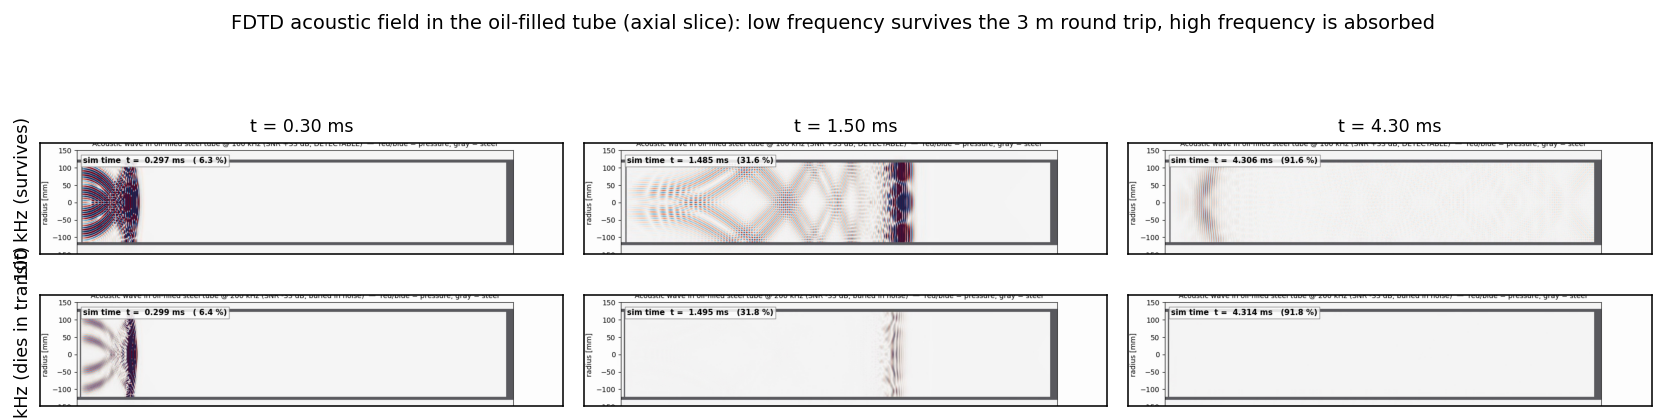
\includegraphics[width=0.99\linewidth]{../figures/fig_wave_montage.png}
\caption{FDTD acoustic field on an axial slice. Top: at 100\,kHz the pulse travels the full
3\,m, reflects, and returns (echo present near the near end at 4.30\,ms). Bottom: at 200\,kHz the
pulse is absorbed before completing the round trip, so no echo returns. The contrast is the
$f^2$ absorption cliff made visible.}
\label{fig:montage}
\end{figure}

\subsection{The receiver, not the channel, is the limit}
The modeled noise floor is dominated by the amplifier voltage noise times the large
thin-film-PZT capacitance (Eq.~\eqref{eq:noise}), giving an output-referred floor of order tens
of millivolts. This is what determines detectability: the same channel against a naive
$10\,\mu$V floor would appear roughly 70\,dB more favorable. The levers that move the boundary
are therefore on the receiver and the frequency, namely a lower transducer capacitance (thicker
or bulk PZT, or charge matching at the element), a quieter front end, a narrower bandwidth or
coded excitation, and above all a lower operating frequency to escape the absorption cliff. A
range-by-frequency feasibility map (Figure~\ref{fig:results}, panel~6) shows the 12\,dB contour
crossing roughly \fbound\,kHz at 3\,m and opening up as either the range shortens or the
frequency drops.

\subsection{Why confinement matters}
A free-field version of the same budget, target at 3\,m in open oil, is dominated by spherical
spreading and is at best marginal and strongly dependent on whether the target is a large
specular reflector or a small scatterer. The tube removes that term: the wave is guided, the far
end reflects nearly all of it, and the geometric penalty reduces to the aperture fill fraction.
This is why a sealed oil-filled tube is a far more forgiving channel than open water, and why the
feasibility question turns on absorption and electronics rather than on spreading.

\section{Limitations and failure modes}
The dominant limitation is absolute calibration. The source paper's transmit deflection
sensitivity, its Eq.~17 receive sensitivity, and its tabulated design-map sensitivities
disagree by more than $100\times$ when cross-checked, so any absolute SNR inherits roughly that
uncertainty. I therefore present the absolute numbers as indicative and rest the conclusions on
the relative structure, which is calibration independent: the $f^2$ cliff, the passivity
constraint, the capacitance-limited noise regime, and the existence and approximate location of
a detection boundary. The FDTD is a two-dimensional axial slice with a reduced steel speed and is
used only for visualization. The oil attenuation and PZT permittivity are representative values,
not measurements of a specific oil or device. There is no physical experiment; this is a modeling
study whose purpose is to set design intuition and to provide a self-consistent, reproducible
budget that a measurement campaign can later anchor.

\section{Conclusion}
For PMUT pulse-echo down a 3\,m oil-filled steel tube, the conventional imaging design point near
1\,MHz fails by a wide margin, because oil absorption over the round trip grows as $f^2$ and
annihilates the echo. Confinement in the tube, not free-field radiation, makes the channel
favorable, and once transmit and receive are tied to one coupling so the link is passive, the
binding constraint is the receiver capacitance and amplifier noise rather than the acoustics. The
usable band is near and below \fbound\,kHz, and the design effort should go into lowering the
operating frequency and the receiver noise floor. The model, the reciprocity relation, the noise
budget, and the visualizations are reproducible from the released code.

\section{Code and data availability}
All code, figures, and the wave-propagation videos are released at
\url{https://github.com/rayjyotir5/pmut-tube-echo}. The repository contains the 1D
link-budget and noise model (\texttt{pmut\_echo\_sim.py}), the 2D FDTD solver and
animation generator (\texttt{pmut\_wave2d.py}), the figure scripts, the rendered
100/135/200 kHz movies, and a README with step-by-step reproduction instructions. The
results figure and reports regenerate with \texttt{python3 pmut\_echo\_sim.py 100 135 200};
each FDTD movie with \texttt{python3 pmut\_wave2d.py <freq\_kHz>}.

\section*{Acknowledgements}
This study, including the derivations, the simulation code, the figures, and the writing of this
paper, was carried out with Claude (Anthropic) acting as an autonomous research and writing
assistant under human direction. The human contribution was the choice of the starting paper, the
physical scenario and a small set of physical parameters, and steering and quality feedback;
the AI contribution was the reading, modeling, coding, debugging, figure generation, and drafting.
A full provenance record appears in Appendix~\ref{app:provenance}.

\bibliographystyle{plainnat}
\bibliography{refs}

\appendix
% ===================== APPENDIX =====================
\section{Provenance: human input versus AI effort}\label{app:provenance}
This work was produced in a single interactive session in which a human supplied the
starting paper, the physical scenario, a small set of physical parameters, and steering and
quality feedback, while an AI agent (Claude, Anthropic, Opus 4.8) performed all reading,
derivation, coding, debugging, figure generation, and writing. I log this explicitly so the
division of labor is preserved.

\subsection{Verbatim human prompts}
Light typographic errors are preserved as written.
\begin{enumerate}\itemsep1pt
\item ``read the modelling.pdf and understand what it is doing, will specify the actual problem after that''
\item ``Has analytical model shown acoustic transmission through 10 mm steel + synthetic mineral oil yields detectable echo at 3 m with SNR $\geq$ 12 dB at 1 MHz centre frequency? if not i want to set up a simulation and visualize the results'' (clarifying choices: pulse-echo through wall; sweep noise; 1D analytical + transfer matrix)
\item ``lets now upgrade the sim to a 2d environment, a steel tube is 3m long, 10mm thick and since it is the cross section of a circular tube, the outer dia of the tube is 300mm. the pmut is positioned at one end and the other end forms the reflecting surface (this end may have increased thickness of steel so as to ignore steel-air interface). tube is filled with oil. now run the simulation and repeat previous sweeps. feel free to re-center the frequency sweep and not assume 1MHz is a fixed input so that SNR is optimal. i'd also like to see a video or gif animation, use the WaveSimulator2D approach if required.''
\item ``oil attenuation is 20 db/m and waveguide wall-bounce loss of 0.5db/m is fine. in the mp4, please render two more panels below the wave propagation animation. one is the pmut transmitter signal over time and a vertical line moves along synced to wave animation. similarly a panel for measured pmut receiver signal. also have a legend to show physical time of sim progress. hope the wave is simulated with noise considered at 250khz''
\item ``erm 20db/m was not at 1mhz, it is at 250khz''
\item ``render a second clip at the $\sim$50-100 kHz optimum so you can see a clean, surviving echo for contrast''
\item ``is the sharp drop at 1MHz in the SNR vs frequency correct? why is this happening? would it help to now stop the sweep and model the noise correctly?''
\item ``yes'' (proceed to tie transmit and receive to one reciprocity-consistent coupling)
\item ``lets now regenerate the results plots and wave propagation animations with the new calibrated model and view it above and below 135kHz''
\item ``make sure to regenerate pmut\_tube\_results.png''
\item ``i dont want three png files, i want a single one''
\item ``the plots are at 250khz, pls update to 100, 135, 200''
\item ``plot y axes are not scaled correctly, getting cropped''
\item ``panel 1 and 4 as well, will log scale help?''
\item ``i dont like the bar chart in panel 4, id rather see the waveform, not normalized to noise''
\item ``treat this entire session as the research done, document everything and produce the resultant paper''
\end{enumerate}

\subsection{Session flow}
Turn 1 established what the source model does. Turn 2 established that it does not address the
ranging question and produced a first free-field link budget (two self-found bugs fixed:
double-counted spreading, and an unphysical multi-watt transmit). Turn 3 reformulated the
channel as a tube waveguide and added the 2D FDTD (a sign-error instability was found and
fixed). Turns 4 to 6 set parameters, built the synchronized three-panel animation, corrected
the attenuation reference frequency (a 112 dB change at the operating point), and rendered a
low-frequency contrast clip. Turn 7 diagnosed the SNR cliff as the $f^2$ absorption law and
replaced the assumed noise floor with a modeled one. Turn 8 tied transmit and receive together
by reciprocity, removing an impossible gain-above-unity artifact. Turns 9 to 15 regenerated all
outputs with the calibrated model and refined figure quality. Turn 16 produced this paper.

\section{Full parameter set}\label{app:params}
All values are documented in the released configuration (\texttt{src/pmut\_echo\_sim.py}).

\begin{table}[h]
\centering\small
\begin{tabular}{lll}
\toprule
Group & Quantity & Value \\
\midrule
Geometry & tube length $L$ & 3.0 m \\
         & outer diameter / wall & 300 mm / 10 mm \\
         & inner oil radius $R_{\mathrm{in}}$ & 140 mm \\
         & effective aperture radius $a_{\mathrm{ap}}$ & 5 mm \\
Steel    & density / speed & 7850 kg/m$^3$ / 5900 m/s \\
         & impedance & 46.3 MRayl \\
Oil      & density / speed & 850 kg/m$^3$ / 1440 m/s \\
         & impedance & 1.22 MRayl \\
         & absorption $\alpha_0$ at 250 kHz & 20 dB/m, $\propto f^2$ \\
         & waveguide wall-bounce loss & 0.5 dB/m \\
         & far-end reflection $\Gamma$ & 0.99 \\
Transducer & quality factor $Q$ & 55 \\
         & $\Lambda', \Lambda_1, \Lambda_2$ & 0.99, 0.33, 0.20 \\
         & $e_{31,f}$ & $-24.24$ C/m$^2$ \\
         & flexural rigidity $D_e$ (calibrated) & $1.0\times10^{-5}$ N\,m \\
         & plate eigenvalue $\alpha_{00}$ & 3.19 \\
         & deflection sens. anchor & 3 nm/V at 500 $\mu$m, 126 kHz \\
Receiver & feedback cap $C_f$ & 10 pF \\
         & amplifier voltage noise $e_n$ & 4 nV/$\sqrt{\text{Hz}}$ \\
         & PZT permittivity / thickness & 1000 / 650 nm \\
         & electrode fill / stray cap & 0.7 / 5 pF \\
         & dielectric loss $\tan\delta$ & 0.02 \\
Operating & drive voltage $V_{\mathrm{in}}$ & 10 V \\
          & detection threshold & 12 dB \\
\bottomrule
\end{tabular}
\caption{Model parameters. Steel speed is reduced to 2500 m/s in the FDTD only (density kept),
to relax the time step while preserving the impedance contrast.}
\end{table}

\section{Derivations}\label{app:derivations}
\paragraph{Wall transfer matrix.} The intensity transmission of a single steel layer of
impedance $Z$ and thickness $d$ between a source medium $Z_1$ and the oil $Z_2$ is
\begin{equation}
\tau_{\mathrm{wall}} = \frac{4 Z_1 Z_2}{(Z_1+Z_2)^2\cos^2(kd) + \big(Z + Z_1 Z_2/Z\big)^2\sin^2(kd)} .
\end{equation}
For a transducer well coupled to steel ($Z_1=Z$) this reduces to the bare interface value
$4 Z_1 Z_2/(Z_1+Z_2)^2 \approx -10$ dB, independent of frequency; for an air-backed transducer
($Z_1=Z_{\mathrm{air}}$) the $\sin^2$ term creates deep nulls between the half-wave resonances
at $n\,c_{\mathrm{steel}}/2d$.

\paragraph{Confinement (fill) factor.} In free space the on-axis far-field pressure of a piston
of radius $a$ falls as $\pi a^2/(\lambda z)$, so the monostatic round trip costs that factor
squared, about $-41$ dB at $z=3$ m. In the tube the launched power instead fills the
cross-section and is conserved (apart from absorption); the only geometric loss is the fraction
the receive aperture re-samples on return, $(a_{\mathrm{ap}}/R_{\mathrm{in}})^2$, which tends to
unity as the aperture fills the tube.

\paragraph{Reciprocity relation.} In the lumped circuit the transformer (ratio $\phi$) maps the
electrical port to the mechano-acoustic port with $P=\phi V$ and $I=\phi\dot q$. Transmit gives
$\dot q = \phi V_{\mathrm{in}}/Z_m$; receive gives $Q = \phi P_{\mathrm{in}}/(j\omega Z_m)$.
Eliminating $\phi$ and $Z_m$ yields Eq.~\eqref{eq:reciprocity}. Anchoring $\dot q/V$ to the
measured 3 nm/V deflection and deriving $Q/P_{\mathrm{in}}$ from it makes the two paths share one
coupling, so the two-way transfer cannot exceed what passivity allows.

\paragraph{Noise.} The output-referred voltage-noise gain of a charge amplifier reading a source
capacitance $C_s$ is $C_{\mathrm{in}}/C_f$ with $C_{\mathrm{in}}=C_s+C_{\mathrm{stray}}+C_f$.
The three terms in Eq.~\eqref{eq:noise} are amplifier voltage noise, amplifier current noise
through the feedback transimpedance $Z_f=1/(\omega C_f)$, and the PZT dielectric-loss Johnson
noise with parallel conductance $G=\omega C_s\tan\delta$, all integrated over
$\mathrm{ENBW}=(\pi/2)(f_0/Q)$.

\paragraph{FDTD update.} The variable-density acoustic field uses a staggered velocity-pressure
leapfrog: $\mathbf{v}\mathrel{-}= (\Delta t/\rho)\nabla p$, then
$p \mathrel{-}= \Delta t\,\rho c^2\,\nabla\!\cdot\mathbf{v}$, stable for
$c_{\max}\Delta t/\Delta x \le 1/\sqrt 2$ in 2D. Open boundaries use a graded sponge layer; oil
absorption is applied as a per-step decay $\exp(-\alpha c\,\Delta t)$ matched to
Eq.~\eqref{eq:absorption} at the operating frequency. A sign error in the velocity update (using
$+\nabla p$) made the scheme blow up; correcting it to $-\nabla p$ restored stability.

\section{Additional results}\label{app:results}
\begin{table}[h]
\centering\small
\begin{tabular}{lrrrrr}
\toprule
$f$ (kHz) & oil loss (dB, RT) & echo & noise floor & SNR (dB) & $V_{\mathrm{echo}}/V_{\mathrm{in}}$ \\
\midrule
75  & 11  & --       & --      & +46  & 0.168 \\
100 & 19  & 479 mV   & 10.2 mV & +33.4 & 0.048 \\
135 & 35  & 57.6 mV  & 11.9 mV & +13.7 & 0.0058 \\
200 & 77  & 0.316 mV & 14.5 mV & $-33.2$ & $3.2\times10^{-5}$ \\
250 & 120 & 1.7 $\mu$V & 16.2 mV & $-79$ & $1.8\times10^{-7}$ \\
1000& 1920 & $\sim$0 & 32 mV   & $-1898$ & $4\times10^{-98}$ \\
\bottomrule
\end{tabular}
\caption{Calibrated link at the design aperture (5 mm) and 3 m range. The detection boundary
(12 dB) sits near 135 kHz. $V_{\mathrm{echo}}/V_{\mathrm{in}}<1$ at every frequency confirms the
model is passive after the reciprocity fix; before the fix it reached 14 at 75 kHz.}
\end{table}

\section{Calibration inconsistency}\label{app:calib}
The source paper reports three sensitivity figures that do not agree when cross-checked. Its
Eq.~17 receive charge sensitivity evaluates to about 1130 fC/Pa for the configured stack, while
the value implied by its measured 3 nm/V transmit deflection through the reciprocity relation is
about 27 fC/Pa, a factor of 41. Separately, its design-map deflection sensitivity (Table 3,
$\sim$0.42 $\mu$m/V) and its measured deflection (Fig.~9, 3 nm/V) differ by more than $100\times$.
I therefore treat absolute SNR as uncertain to roughly two orders of magnitude and rest the
conclusions on the calibration-independent structure: the $f^2$ cliff, passivity, the
capacitance-limited noise regime, and the existence of a detection boundary. Under any
self-consistent choice within this spread, 250 kHz and above fail and the usable band is at low
frequency.

\section{Reproducibility}\label{app:repro}
\begin{verbatim}
cd src
python3 pmut_echo_sim.py 100 135 200   # -> ../figures/pmut_tube_results.png + reports
python3 pmut_wave2d.py 100             # -> 100khz.mp4/.gif  (also 135, 200)
python3 make_paper_figures.py          # -> schematic + wave montage
cd ../paper
pdflatex main && bibtex main && pdflatex main && pdflatex main
\end{verbatim}
Environment: Python 3.11, NumPy 2.0, SciPy 1.14, Matplotlib 3.10, imageio with the ffmpeg
plugin; TeX Live 2025. The 1D link budget runs in seconds; each FDTD clip is a few minutes on a
single CPU core.

\section{AI involvement checklist (summary)}\label{app:checklist}
Research stage assessment: ideation and framing were human-seeded (the scenario and the ranging
question) and AI-developed; the literature anchor (one paper) was human-provided; experiment
design, implementation, analysis, and writing were AI-led with human steering and feedback (High
AI involvement). AI systems used: Claude (Anthropic), Opus 4.8, as an agent with code execution
and figure generation. Known limitations and failure modes are stated in the main text
(Limitations) and Appendix~\ref{app:calib}: absolute calibration uncertainty, a visualization-only
2D solver, representative rather than measured material properties, and the absence of a physical
experiment.


\end{document}
